\documentclass[aspectratio=169,11pt]{beamer}
\usepackage{beamerucad}
\usepackage{listings}
\definecolor{ckw}{HTML}{2563AB}\definecolor{cst}{HTML}{2E8B57}\definecolor{ccm}{HTML}{8A8F98}
\lstdefinestyle{py}{language=Python,basicstyle=\ttfamily\footnotesize,
 keywordstyle=\color{ckw}\bfseries,stringstyle=\color{cst},commentstyle=\color{ccm}\itshape,
 showstringspaces=false,columns=fullflexible,keepspaces=true,
 backgroundcolor=\color{ucadband!8},frame=leftline,framerule=2.5pt,rulecolor=\color{ucadband},
 xleftmargin=8pt,aboveskip=3pt,belowskip=1pt,basewidth=0.5em}
\lstset{style=py}
\title{Introduction au ML — Séance 5}
\subtitle{Prédire un nombre : la régression linéaire, de l'équation normale à Ridge}
\author{Dr. El Hadji Bassirou TOURÉ}
\institute{Département de Mathématiques et Informatique\\ Faculté des Sciences et Techniques\\ Université Cheikh Anta Diop de Dakar}
\date{}
\setucadfoot{Introduction au ML --- Séance 5}
\graphicspath{{figs/}}
\begin{document}

\begin{frame}[plain,noframenumbering]\titlepage\end{frame}

\begin{frame}{Objectifs de la séance}
\begin{ucaddef}[Contenu]
{\small Cette séance construit le deuxième pilier du cours : prédire une \textbf{quantité} continue. Elle introduit le modèle linéaire, deux façons de l'entraîner — l'\textbf{équation normale} et la \textbf{descente de gradient} — puis les outils pour l'évaluer et le discipliner.}
\end{ucaddef}
\begin{itemize}\small
  \item Formuler la \textbf{régression} : la fonction $f$, la droite $\hat y = b + w\,x$, les résidus.
  \item Définir la \textbf{meilleure droite} par la \textbf{MSE}, et la calculer exactement : l'\textbf{équation normale}.
  \item Apprendre par itérations : la \textbf{descente de gradient}, pas calculés à la main, rôle du pas $\eta$.
  \item Lire \textbf{MAE}, \textbf{RMSE} et \textbf{R²} ; diagnostiquer par les résidus.
  \item Le degré d'un polynôme comme bouton de complexité ; la \textbf{courbe en U} ; \textbf{Ridge} pour dompter le sur-ajustement.
\end{itemize}
\end{frame}

% #####################################################################
\section[Prédire : le modèle linéaire]{Prédire une quantité : le modèle linéaire}

\begin{frame}{La régression : prédire un nombre}
\begin{ucadfront}[Changement de question]
{\small Les Séances 3 et 4 prédisaient une \emph{classe} (séjour long ou court, oui ou non). La direction de l'hôpital de Thiès pose une autre question : \textbf{combien de jours} ce patient restera-t-il ? Une classe ne suffit plus — il faut un \textbf{nombre}.}
\end{ucadfront}
\ucadformula{f : \mathcal{X} \longrightarrow \mathbb{R}, \qquad f(x_i) \approx y_i}
{\small La \textbf{régression} est l'apprentissage supervisé dont la sortie est un réel : à partir d'exemples étiquetés $(x_i, y_i)$ avec $y_i \in \mathbb{R}$, $f$ ne choisit plus une étiquette, elle renvoie une valeur sur un axe continu. Ici $\mathcal{X} \subset \mathbb{R}^{5}$ (âge, glycémie, hémoglobine, fièvre, saison) et la cible $y$ est la \textbf{durée d'hospitalisation} en jours. Même protocole qu'en Séance 3 — \texttt{fit}/\texttt{predict}, train/test — seul l'espace de sortie change : $\mathcal{Y} = \mathbb{R}$ au lieu de $\{0,1\}$, et l'erreur se mesure en \emph{distance} ($\hat y - y$), non plus en correct/incorrect.}
\end{frame}

\begin{frame}{Les données : $X$ et un $y$ devenu réel}
\begin{ucadex}[Premières lignes réelles de DataSANTÉ-221]
{\footnotesize \renewcommand{\arraystretch}{1.0}\begin{tabular}{c|ccccc|c}
 & âge & glycémie & hémoglobine & fièvre & saison & durée (j)\\\hline
$x_1$ & $47$ & $9{,}3$ & $11{,}8$ & $38{,}0$ & $0$ & $y_1 = 3{,}8$\\
$x_2$ & $18$ & $5{,}1$ & $13{,}0$ & $39{,}5$ & $1$ & $y_2 = 0{,}5$\\
$x_3$ & $56$ & $7{,}2$ & $9{,}5$ & $37{,}1$ & $1$ & $y_3 = 6{,}5$\\
\end{tabular}}
\vspace{2pt}

{\footnotesize \[ X=\begin{pmatrix} 47 & 9{,}3 & 11{,}8 & 38{,}0 & 0\\ 18 & 5{,}1 & 13{,}0 & 39{,}5 & 1\\ 56 & 7{,}2 & 9{,}5 & 37{,}1 & 1\\ \vdots & \vdots & \vdots & \vdots & \vdots \end{pmatrix} \in \mathbb{R}^{10000\times 5} \qquad y=\begin{pmatrix} 3{,}8\\ 0{,}5\\ 6{,}5\\ \vdots \end{pmatrix} \in \mathbb{R}^{10000} \]}
\end{ucadex}
{\small La matrice de design $X$ est inchangée depuis la Séance 3 ; la seule nouveauté est dans $y$, qui vit désormais dans $\mathbb{R}^{n}$ et non dans $\{0,1\}^{n}$.}
\end{frame}

\begin{frame}{Exercice — régression ou classification ?}
\begin{ucadrec}[Énoncé]
{\small Pour chaque problème, déterminer s'il relève de la régression ou de la classification : \textbf{(a)} prédire le rendement d'un champ de mil à Kaolack (en tonnes/ha) ; \textbf{(b)} prédire si une transaction mobile money est frauduleuse ; \textbf{(c)} prédire la glycémie d'un patient dans six mois ; \textbf{(d)} prédire la gravité d'un cas parmi \{bénin, modéré, sévère\}.}
\end{ucadrec}
\pause
\begin{ucadex}[Correction]
{\small \textbf{(a)} régression — la sortie est un réel ; \textbf{(b)} classification binaire ; \textbf{(c)} régression — un nombre, même si l'entrée contient l'ancienne glycémie ; \textbf{(d)} classification à trois classes : les modalités sont \emph{ordonnées} mais restent des catégories, pas des quantités continues.}
\end{ucadex}
\end{frame}

\begin{frame}{L'idée : une droite qui suit le nuage}
\begin{ucadfront}[Analogie]
{\small Le prix d'une course de taxi à Dakar : une \emph{prise en charge} fixe, puis un tarif \emph{par kilomètre}. Le modèle linéaire fait de chaque prédiction une course de taxi : un point de départ $b$, et un prix $w_j$ par unité de chaque caractéristique.}
\end{ucadfront}
\figslideb{0.95}{f5_fit}{Même nuage, deux droites de qualités différentes : le carré $\hat y_i$ est posé \emph{sur} la droite, le tiret rouge est le \textbf{résidu} $y_i-\hat y_i$ ; la bonne droite serre les résidus.}
\end{frame}

\begin{frame}{Le modèle linéaire, formellement}
\begin{ucaddef}[Définition]
{\small Le \textbf{modèle linéaire} prédit par une somme pondérée des caractéristiques : chaque variable contribue proportionnellement à son poids, et $b$ fixe le niveau de base.}
\end{ucaddef}
\ucadformula{\hat y \;=\; b + w_1 x_1 + w_2 x_2 + \cdots + w_d x_d \;=\; b + \mathbf{w}\cdot \mathbf{x}}
{\small $\mathbf{w} = (w_1,\dots,w_d)$ est le vecteur des \textbf{poids} (un par caractéristique) et $b$ l'\textbf{ordonnée à l'origine} (\emph{intercept}) : la prédiction quand toutes les caractéristiques valent $0$. Apprendre, c'est choisir les $d+1$ nombres $(b, w_1, \dots, w_d)$ — rien d'autre. Avec une seule variable, le modèle est la droite $\hat y = b + w\,x$.}
\end{frame}

\begin{frame}{Exemple — évaluer $\hat y$ terme à terme}
\begin{ucadex}[Le patient $x_1$ passe dans le modèle]
{\small Modèle entraîné sur DataSANTÉ-221 (coefficients réels, arrondis) : $b = 0{,}64$, puis par variable :
\begin{center}\footnotesize\renewcommand{\arraystretch}{1.05}\begin{tabular}{l|ccccc}
 & âge & glycémie & hémoglobine & fièvre & saison\\\hline
poids $w_j$ & $0{,}048$ & $0{,}566$ & $-0{,}263$ & $0{,}011$ & $1{,}379$\\
valeur $x_{1j}$ & $47$ & $9{,}3$ & $11{,}8$ & $38{,}0$ & $0$\\
produit $w_j x_{1j}$ & $2{,}27$ & $5{,}26$ & $-3{,}11$ & $0{,}41$ & $0$\\
\end{tabular}\end{center}
$\hat y_1 = 0{,}64 + 2{,}27 + 5{,}26 - 3{,}11 + 0{,}41 + 0 = \mathbf{5{,}48}$ jours. La durée réelle est $y_1 = 3{,}8$ : résidu $= 3{,}8 - 5{,}48 = -1{,}68$ jour — le modèle surestime ce patient.}
\end{ucadex}
\end{frame}

\begin{frame}{Lire les coefficients : chaque poids est une pente}
\begin{columns}[c]
\column{0.54\linewidth}
\begin{ucaddef}[L'idée en une phrase]
{\small Chaque poids $w_j$ est un \textbf{taux de changement} : « une unité de plus sur la variable $j$ déplace la prédiction de $w_j$ » (toutes choses égales par ailleurs).}
\end{ucaddef}
{\small Sur la durée d'hospitalisation :}
\begin{itemize}\small
  \item glycémie $w = +0{,}57$ : $+1$ mmol/L ajoute $\approx$ une demi-journée ;
  \item saison $w = +1{,}38$ : l'hivernage ajoute $1{,}4$ jour ;
  \item hémoglobine $w = -0{,}26$ : meilleure hémoglobine, séjour plus court.
\end{itemize}
\column{0.44\linewidth}
\centering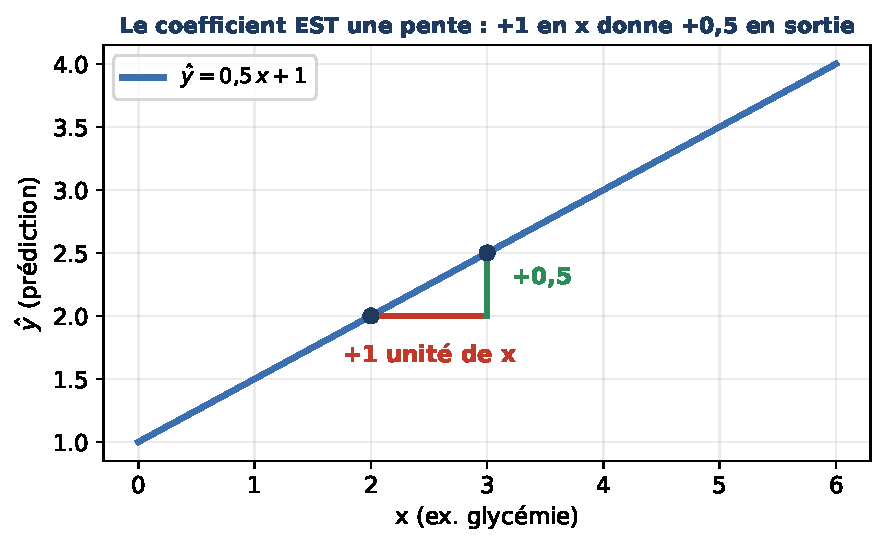
\includegraphics[width=\linewidth]{f5_coef_slope}
\end{columns}
\vspace{2pt}

{\footnotesize \textbf{Piège.} Comparer la \emph{taille} de deux coefficients n'a de sens que sur la \textbf{même échelle} (Séance 4) ; et un poids décrit une \emph{association}, pas une cause.}
\end{frame}

\begin{frame}{Exercice — manier les coefficients}
\begin{ucadrec}[Énoncé]
{\small Avec le modèle ci-dessus ($w_{\text{glycémie}} = 0{,}566$, $w_{\text{saison}} = 1{,}379$) : \textbf{(a)} de combien la durée prédite change-t-elle si la glycémie augmente de $2$ mmol/L, le reste étant inchangé ? \textbf{(b)} et si, de plus, on passe de la saison sèche ($0$) à l'hivernage ($1$) ?}
\end{ucadrec}
\pause
\begin{ucadex}[Correction]
{\small \textbf{(a)} $\Delta\hat y = 0{,}566 \times 2 = \mathbf{+1{,}13}$ jour. \textbf{(b)} s'y ajoute $1{,}379 \times 1$, soit au total $1{,}13 + 1{,}38 = \mathbf{+2{,}51}$ jours. La linéarité rend ces effets \emph{additifs} : chaque variable pousse la prédiction indépendamment des autres.}
\end{ucadex}
\end{frame}

% #####################################################################
\section[La meilleure droite]{La meilleure droite : la MSE}

\begin{frame}{Que veut dire la meilleure droite ?}
\begin{ucaddef}[L'idée en une phrase]
{\small Une droite est bonne si ses erreurs verticales — les \textbf{résidus} $y_i - \hat y_i$ — sont petites ; la meilleure droite est celle qui rend ces erreurs \emph{globalement} les plus petites possibles.}
\end{ucaddef}
{\small Il faut donc une règle qui transforme $n$ résidus en \textbf{un seul nombre} à minimiser. La convention du ML : élever chaque résidu au carré (les signes ne se compensent plus, les grandes erreurs pèsent lourd), puis moyenner.}
\end{frame}

\begin{frame}{L'erreur quadratique moyenne, formellement}
\begin{ucaddef}[Définition]
{\small La \textbf{MSE} (\emph{mean squared error}) d'un modèle est la moyenne des carrés de ses résidus. Entraîner une régression linéaire, c'est chercher les paramètres qui la minimisent : le critère des \textbf{moindres carrés}.}
\end{ucaddef}
\ucadformula{J(b,\mathbf{w}) \;=\; \frac{1}{n}\sum_{i=1}^{n}\big(y_i - \hat y_i\big)^2 \qquad\qquad (\hat b,\hat{\mathbf{w}}) \;=\; \arg\min_{b,\mathbf{w}}\; J(b,\mathbf{w})}
{\small Chaque terme $(y_i - \hat y_i)^2$ est le carré d'un résidu ; la somme agrège, la division par $n$ moyenne. $J$ dépend des \emph{paramètres} (les données sont fixées) : changer $(b,\mathbf{w})$ déplace la droite et change $J$. Le carré rend $J$ \textbf{lisse} et en forme de \textbf{cuvette} — propriété décisive pour la suite.}
\end{frame}

\begin{frame}{Exemple — comparer deux droites par leur MSE}
\centering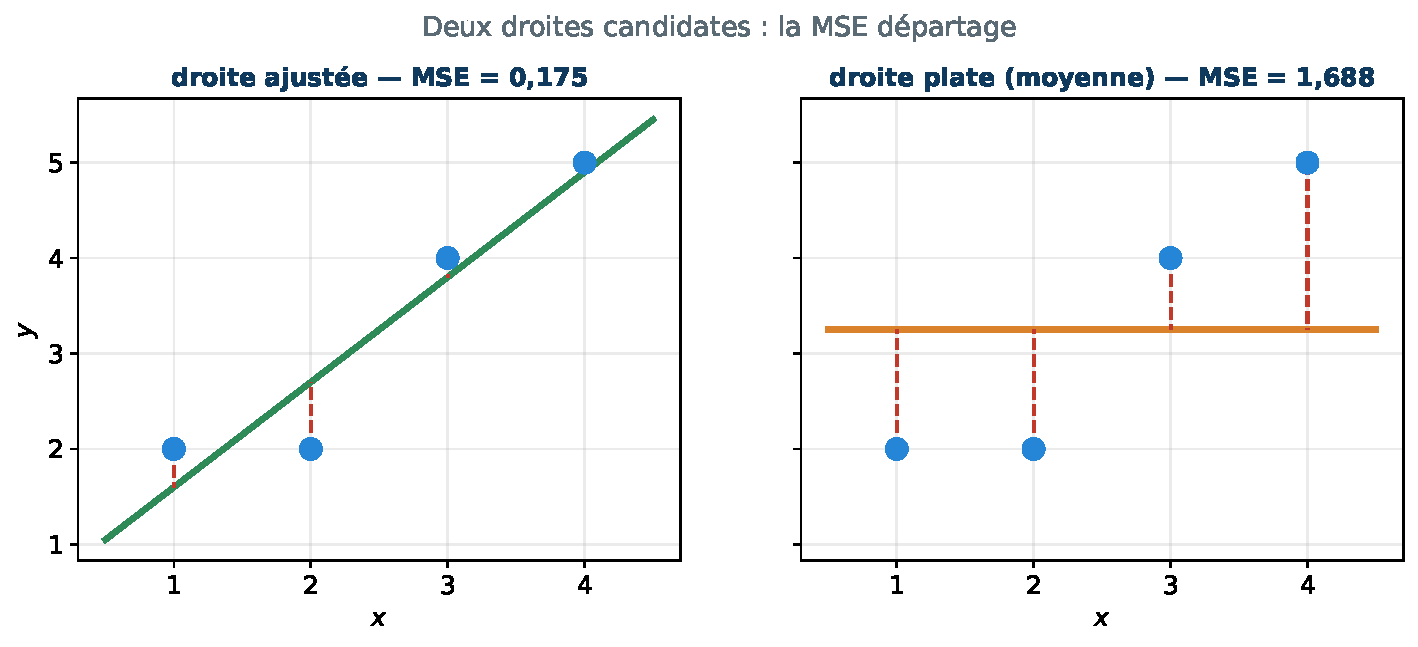
\includegraphics[width=0.78\linewidth]{f5_two_lines}
\vspace{-1pt}

{\small Jouet : $x = [1,2,3,4]$, $y = [2,2,4,5]$. À gauche, $\hat y = 0{,}5 + 1{,}1\,x$ : résidus $(0{,}4;\,-0{,}7;\,0{,}2;\,0{,}1)$, carrés $(0{,}16;\,0{,}49;\,0{,}04;\,0{,}01)$, MSE $= 0{,}70/4 = \mathbf{0{,}175}$. À droite, la droite plate $\hat y = \bar y = 3{,}25$ : MSE $= \mathbf{1{,}688}$ — dix fois pire.}
\end{frame}

\begin{frame}{Exercice — calculer la MSE de la droite plate}
\begin{ucadrec}[Énoncé]
{\small Vérifier la valeur $1{,}688$ : calculer les quatre résidus de la droite $\hat y = 3{,}25$ sur le jouet $y = [2,2,4,5]$, leurs carrés, puis la MSE.}
\end{ucadrec}
\pause
\begin{ucadex}[Correction]
{\small Résidus : $2-3{,}25 = -1{,}25$ ; $-1{,}25$ ; $0{,}75$ ; $1{,}75$. Carrés : $1{,}5625$ ; $1{,}5625$ ; $0{,}5625$ ; $3{,}0625$. Somme $= 6{,}75$, MSE $= 6{,}75/4 = \mathbf{1{,}6875}$. À noter : ce $6{,}75$ resservira tel quel dans le calcul du R².}
\end{ucadex}
\end{frame}

% #####################################################################
\section[L'équation normale]{L'équation normale : le minimum exact}

\begin{frame}{Le cas d'une variable, formellement}
\begin{ucaddef}[L'idée en une phrase]
{\small La MSE est une cuvette parfaitement régulière : au fond, la pente est nulle dans toutes les directions — et ce point d'équilibre se calcule \textbf{directement} à partir des données, sans tâtonner. À une variable, il se lit dans les écarts aux moyennes $\bar x$ et $\bar y$.}
\end{ucaddef}
\ucadformula{\hat w \;=\; \frac{\sum_i (x_i - \bar x)(y_i - \bar y)}{\sum_i (x_i - \bar x)^2}\,, \qquad \hat b \;=\; \bar y - \hat w\,\bar x}
{\small Le numérateur de $\hat w$ mesure comment $x$ et $y$ \emph{varient ensemble} ; le dénominateur, combien $x$ varie tout seul. Une fois la pente connue, $\hat b$ cale la droite pour qu'elle passe exactement par le centre de gravité $(\bar x, \bar y)$ du nuage.}
\end{frame}

\begin{frame}{Exemple — la droite calculée à la main}
\begin{ucadex}[Sur les quatre patients du jouet]
{\footnotesize $x=[1,2,3,4]$, $y=[2,2,4,5]$ ; moyennes $\bar x = 2{,}5$, $\bar y = 3{,}25$.
\begin{center}\renewcommand{\arraystretch}{0.95}\begin{tabular}{c|cccc}
$i$ & $x_i - \bar x$ & $y_i - \bar y$ & produit & $(x_i-\bar x)^2$\\\hline
$1$ & $-1{,}5$ & $-1{,}25$ & $+1{,}875$ & $2{,}25$\\
$2$ & $-0{,}5$ & $-1{,}25$ & $+0{,}625$ & $0{,}25$\\
$3$ & $+0{,}5$ & $+0{,}75$ & $+0{,}375$ & $0{,}25$\\
$4$ & $+1{,}5$ & $+1{,}75$ & $+2{,}625$ & $2{,}25$\\\hline
$\Sigma$ & & & $\mathbf{5{,}5}$ & $\mathbf{5{,}0}$\\
\end{tabular}\end{center}
$\hat w = 5{,}5/5{,}0 = \mathbf{1{,}1}$, \quad $\hat b = 3{,}25 - 1{,}1\times 2{,}5 = \mathbf{0{,}5}$ — la droite verte des diapositives précédentes. \texttt{scikit-learn} confirme : \texttt{coef\_} $= 1{,}1$, \texttt{intercept\_} $= 0{,}5$.}
\end{ucadex}
\end{frame}

\begin{frame}{L'équation normale, formellement}
\begin{ucaddef}[Définition]
{\small En dimension quelconque, on absorbe $b$ dans les poids en ajoutant à $X$ une \textbf{colonne de 1} ; le minimum de la MSE est alors donné par une formule matricielle unique : l'\textbf{équation normale}.}
\end{ucaddef}
\ucadformula{\tilde X = \begin{pmatrix} 1 & x_1^{\top}\\ \vdots & \vdots\\ 1 & x_n^{\top} \end{pmatrix}, \qquad \hat\theta \;=\; \big(\tilde X^{\top}\tilde X\big)^{-1}\,\tilde X^{\top} y, \qquad \hat\theta = (\hat b, \hat w_1, \dots, \hat w_d)}
{\small Lecture terme à terme : $\tilde X^{\top} y$ confronte chaque colonne aux cibles (qui co-varie avec $y$) ; $\tilde X^{\top}\tilde X$ enregistre comment les colonnes varient entre elles ; l'inverse $(\cdot)^{-1}$ démêle leurs contributions. Cette formule \emph{est} le point où toutes les pentes de $J$ s'annulent — on l'admet, et on va la \textbf{vérifier} sur le jouet.}
\end{frame}

\begin{frame}{Exemple — l'équation normale sur le jouet, étape 1}
\begin{ucadex}[Construire les deux blocs]
{\small Jouet à une variable : la matrice augmentée $\tilde X$ a deux colonnes (les 1, puis $x$).
\[ \tilde X = \begin{pmatrix} 1 & 1\\ 1 & 2\\ 1 & 3\\ 1 & 4 \end{pmatrix}, \qquad
\tilde X^{\top}\tilde X = \begin{pmatrix} 4 & 10\\ 10 & 30 \end{pmatrix}, \qquad
\tilde X^{\top} y = \begin{pmatrix} 13\\ 38 \end{pmatrix} \]
Chaque case se lit : $4 = $ nombre de patients, $10 = \sum x_i$, $30 = \sum x_i^2$ ; côté cibles, $13 = \sum y_i$ et $38 = \sum x_i y_i$. Tout est déjà là : effectifs, sommes, co-variations.}
\end{ucadex}
\end{frame}

\begin{frame}{Exemple — l'équation normale sur le jouet, étape 2}
\begin{ucadex}[Inverser puis multiplier]
{\small Inverse d'une matrice $2\times 2$ : échanger la diagonale, changer le signe du reste, diviser par le déterminant $4\times 30 - 10\times 10 = \mathbf{20}$ :
\[ \big(\tilde X^{\top}\tilde X\big)^{-1} = \frac{1}{20}\begin{pmatrix} 30 & -10\\ -10 & 4 \end{pmatrix} = \begin{pmatrix} 1{,}5 & -0{,}5\\ -0{,}5 & 0{,}2 \end{pmatrix} \]
\[ \hat\theta = \begin{pmatrix} 1{,}5 & -0{,}5\\ -0{,}5 & 0{,}2 \end{pmatrix}\begin{pmatrix} 13\\ 38 \end{pmatrix} = \begin{pmatrix} 1{,}5\times 13 - 0{,}5\times 38\\ -0{,}5\times 13 + 0{,}2\times 38 \end{pmatrix} = \begin{pmatrix} \mathbf{0{,}5}\\ \mathbf{1{,}1} \end{pmatrix} \]
Le même $(\hat b, \hat w) = (0{,}5\,;\,1{,}1)$ que les formules fermées — l'équation normale les généralise à $d$ variables. \texttt{LinearRegression} applique exactement ce calcul.}
\end{ucadex}
\end{frame}

\begin{frame}{Exercice — résoudre une équation normale}
\begin{ucadrec}[Énoncé]
{\small Sur un autre jeu, on a calculé $\tilde X^{\top}\tilde X = \begin{pmatrix} 2 & 3\\ 3 & 5 \end{pmatrix}$ et $\tilde X^{\top} y = \begin{pmatrix} 4\\ 7 \end{pmatrix}$. Calculer $\hat\theta = (\hat b, \hat w)$.}
\end{ucadrec}
\pause
\begin{ucadex}[Correction]
{\small Déterminant $= 2\times 5 - 3\times 3 = 1$, donc l'inverse est $\begin{pmatrix} 5 & -3\\ -3 & 2 \end{pmatrix}$. Produit : $\hat b = 5\times 4 - 3\times 7 = \mathbf{-1}$ et $\hat w = -3\times 4 + 2\times 7 = \mathbf{2}$. La droite des moindres carrés est $\hat y = -1 + 2x$.}
\end{ucadex}
\end{frame}

\begin{frame}{Piège — quand l'inversion se dérobe}
\begin{ucadpiege}[Deux limites de la solution exacte]
{\small \textbf{Colinéarité} : si une colonne de $X$ est (presque) une combinaison des autres — le poids en kg \emph{et} en livres — alors $\tilde X^{\top}\tilde X$ n'est pas inversible : une infinité de droites donnent la même MSE, le calcul devient instable. \textbf{Coût} : inverser une matrice $(d+1)\times(d+1)$ devient lourd quand $d$ se compte en milliers.}
\end{ucadpiege}
{\small Dans les deux cas, la parade est la même : renoncer au calcul exact et \textbf{approcher} le minimum par petits pas. C'est la descente de gradient — la méthode d'apprentissage la plus importante de tout le ML, des droites aux réseaux de neurones.}
\end{frame}

% #####################################################################
\section{La descente de gradient}

\begin{frame}{La dérivée : mesurer une pente}
\begin{ucaddef}[Pourquoi, et l'idée en une phrase]
{\small L'équation normale exige d'\textbf{inverser une matrice} — impraticable en grande dimension, impossible pour les réseaux. On cherche alors le minimum \emph{à tâtons} (la \textbf{descente de gradient}), et pour « descendre » on mesure une pente : la \textbf{dérivée} $f'(x)$, taux de changement de $f$. Positive, $f$ monte ; négative, $f$ descend ; \textbf{nulle}, on est au creux.}
\end{ucaddef}
\figslideb{0.40}{f5_derivative}{Pente $-4$ (descend), $+4$ (monte), $\mathbf{0}$ au creux : \emph{le minimum est là où la dérivée s'annule}.}
\end{frame}

\begin{frame}{Dérivées partielles et gradient}
\begin{ucaddef}[Une pente par variable, un vecteur pour les réunir]
{\small Quand $f$ dépend de plusieurs variables, la \textbf{dérivée partielle} $\partial f/\partial x$ mesure le taux de changement selon \emph{une seule} composante, les autres figées (sur une colline : la pente vers l'est, pas vers le nord). Le \textbf{gradient} $\nabla f = \big(\partial f/\partial x,\ \partial f/\partial y\big)$ rassemble toutes ces pentes en un \textbf{vecteur} qui pointe vers la \emph{plus forte montée} ; sa longueur dit à quel point ça monte.}
\end{ucaddef}
\figslideb{0.52}{f5_gradient}{$\nabla f=(4;2)$ (vert) pointe vers la plus forte montée ; on descend dans le sens opposé $-\nabla f$ (orange).}
\end{frame}

\begin{frame}{La perte est une cuvette : descendre pas à pas}
\begin{ucaddef}[Pourquoi la descente marche ici]
{\small La MSE de la régression linéaire est \textbf{convexe} : sa surface est une \emph{cuvette} à \textbf{un seul} creux. D'où qu'on vienne, suivre la pente vers le bas mène \emph{toujours} au même fond — le minimum global. C'est la stratégie d'une randonneuse dans le brouillard : sentir la pente, faire un pas vers le bas, recommencer ; la pente locale suffit.}
\end{ucaddef}
\figslideb{0.44}{f5_convex}{Convexe (gauche) : un seul creux. Non convexe (droite) : plusieurs creux (le cas des réseaux, Séance 10).}
\end{frame}

\begin{frame}{La règle de mise à jour, formellement}
\begin{ucaddef}[Définition]
{\small On applique au critère $J$ le gradient qu'on vient de définir : $\nabla J$ pointe vers la plus forte montée de l'erreur ; la règle de mise à jour avance dans le sens \emph{opposé}, d'un pas de taille $\eta$.}
\end{ucaddef}
\ucadformula{\theta^{(t+1)} \;=\; \theta^{(t)} \;-\; \eta\,\nabla J\big(\theta^{(t)}\big), \qquad \theta = (b, \mathbf{w})}
{\small Le signe « $-$ » est tout l'algorithme : le gradient montre la montée, on prend son opposé pour descendre. Le \textbf{pas d'apprentissage} $\eta$ (\emph{learning rate}) dose la prudence : la randonneuse fait-elle des pas de fourmi ou des bonds ? On répète jusqu'à ce que le gradient devienne quasi nul — le fond de la cuvette.}
\end{frame}

\begin{frame}{Le gradient de la MSE, formellement}
\begin{ucaddef}[Les deux pentes de la cuvette]
{\small Pour la droite $\hat y = b + w\,x$, le gradient de la MSE a une forme remarquablement lisible : ce sont des \textbf{moyennes de résidus}.}
\end{ucaddef}
\ucadformula{\frac{\partial J}{\partial b} \;=\; -\frac{2}{n}\sum_{i=1}^{n} r_i\,, \qquad \frac{\partial J}{\partial w} \;=\; -\frac{2}{n}\sum_{i=1}^{n} x_i\, r_i\,, \qquad r_i = y_i - \hat y_i}
{\small (Rappel juste-à-temps : dériver $(y_i - b - w x_i)^2$ par $b$ donne $-2(y_i - b - w x_i)$ — la règle de la fonction composée, rien de plus.) Lecture : si les résidus sont en moyenne positifs, le modèle prédit trop bas $\Rightarrow$ la pente sur $b$ est négative $\Rightarrow$ la mise à jour \emph{augmente} $b$. Le gradient transforme les erreurs en correction.}
\end{frame}

\begin{frame}{Exemple — l'itération 1, à la main}
\begin{ucadex}[Départ au point zéro]
{\small Jouet, départ $(b,w) = (0,0)$, pas $\eta = 0{,}1$. Le modèle prédit $\hat y_i = 0$ partout, donc $r = y = (2,2,4,5)$.
\begin{align*}
\frac{\partial J}{\partial b} &= -\tfrac{2}{4}(2+2+4+5) = -\tfrac{2}{4}\times 13 = \mathbf{-6{,}5}\\[1pt]
\frac{\partial J}{\partial w} &= -\tfrac{2}{4}(1\!\cdot\!2+2\!\cdot\!2+3\!\cdot\!4+4\!\cdot\!5) = -\tfrac{2}{4}\times 38 = \mathbf{-19}
\end{align*}
Mise à jour : $b = 0 - 0{,}1\times(-6{,}5) = \mathbf{0{,}65}$ ; $w = 0 - 0{,}1\times(-19) = \mathbf{1{,}9}$. La MSE chute de $12{,}25$ à $\mathbf{5{,}60}$ : un seul pas, déjà moitié moins d'erreur.}
\end{ucadex}
\end{frame}

\begin{frame}{Exemple — itérations 2 et 3 : le zigzag}
\begin{ucadex}[La correction se corrige]
{\small Au point $(0{,}65\,;\,1{,}9)$, la droite est devenue \emph{trop pentue} : les résidus changent de signe, le gradient s'inverse.
\begin{center}\footnotesize\renewcommand{\arraystretch}{1.05}\begin{tabular}{c|cc|cc|c}
it. & $\partial J/\partial b$ & $\partial J/\partial w$ & $b$ & $w$ & $J$\\\hline
$1$ & $-6{,}5$ & $-19$ & $0{,}65$ & $1{,}9$ & $5{,}60$\\
$2$ & $+4{,}3$ & $+12{,}75$ & $0{,}22$ & $0{,}625$ & $2{,}61$\\
$3$ & $-2{,}94$ & $-8{,}53$ & $0{,}51$ & $1{,}48$ & $1{,}27$\\
\end{tabular}\end{center}
Le trajet \textbf{zigzague} de part et d'autre du minimum — sur-correction, contre-correction — mais chaque rebond est plus petit que le précédent, et $J$ ne cesse de baisser.}
\end{ucadex}
\end{frame}

\begin{frame}{La trajectoire et la convergence}
\begin{columns}[c]
\column{0.45\linewidth}
\centering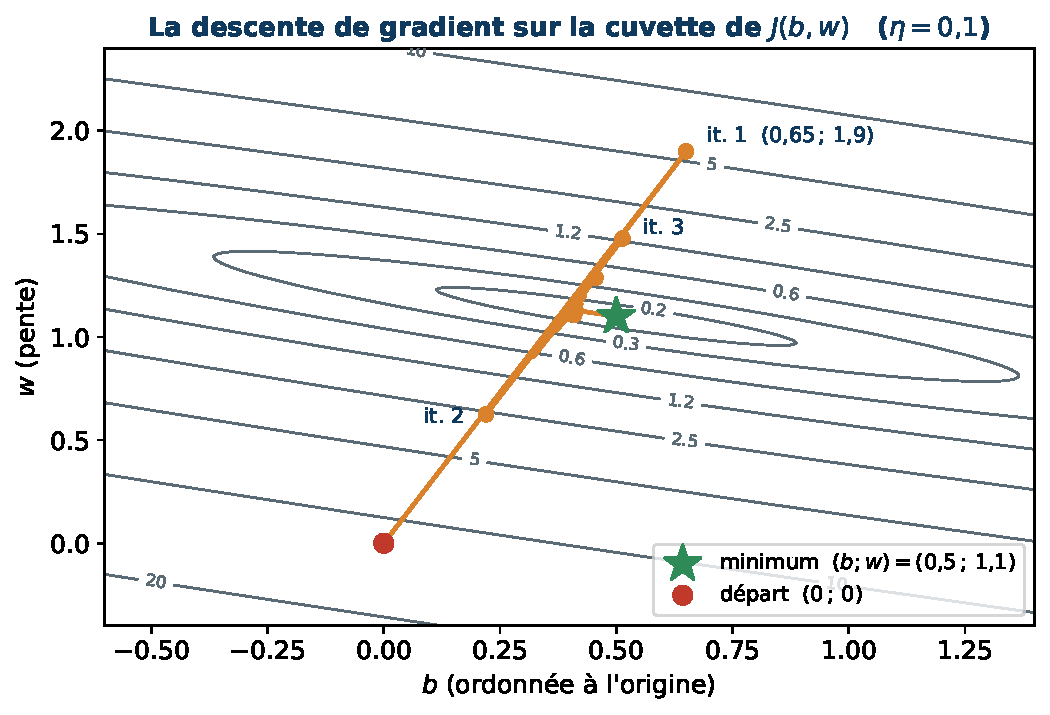
\includegraphics[width=\linewidth]{f5_bowl}
\column{0.55\linewidth}
\begin{ucadex}[Du zigzag au minimum exact]
{\small Itérations, $\eta = 0{,}1$ :
\begin{center}\footnotesize\renewcommand{\arraystretch}{1.05}\begin{tabular}{c|ccc}
it. & $b$ & $w$ & $J$\\\hline
$10$ & $0{,}410$ & $1{,}107$ & $0{,}180$\\
$100$ & $0{,}495$ & $1{,}102$ & $0{,}175$\\
$300$ & $0{,}500$ & $1{,}100$ & $0{,}175$\\
\end{tabular}\end{center}
À l'itération 300, la descente retrouve $(0{,}5\,;\,1{,}1)$ et $J = 0{,}175$ : \textbf{exactement} la solution de l'équation normale.}
\end{ucadex}
\end{columns}
\vspace{2pt}

{\scriptsize Courbes de niveau de $J(b,w)$ : départ rouge en $(0;0)$, zigzag orange, convergence vers l'étoile $(0{,}5\,;\,1{,}1)$. Deux chemins, un même fond — la cuvette garantit qu'aucun autre creux ne piège la descente.}
\end{frame}

\begin{frame}{Le pas $\eta$ décide de tout}
\centering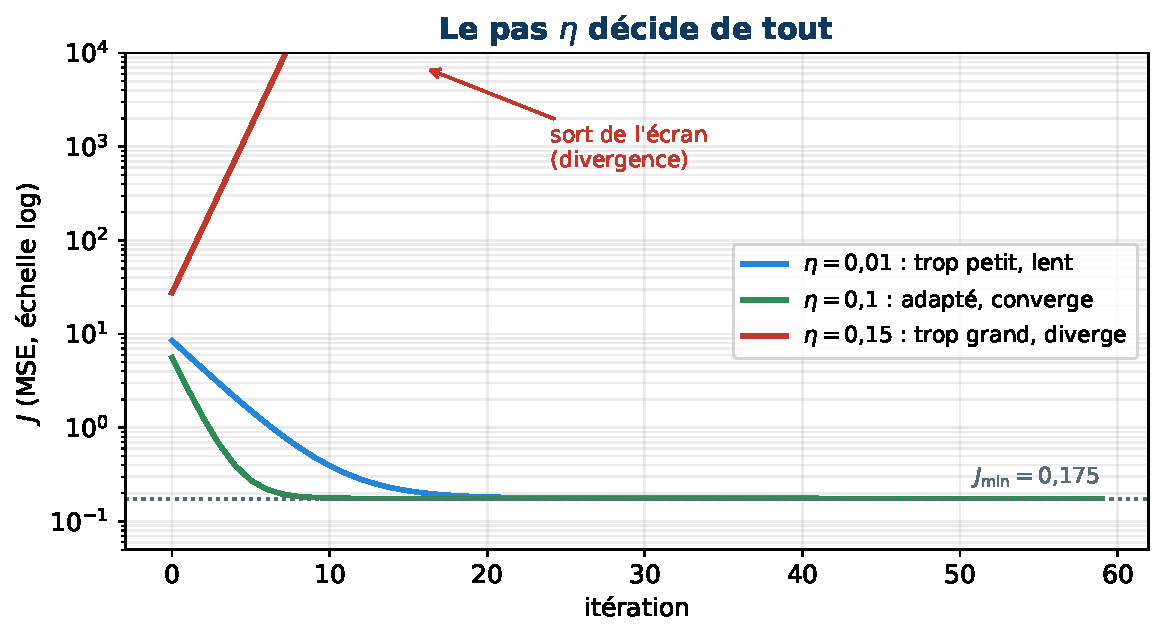
\includegraphics[width=0.60\linewidth]{f5_eta}
\vspace{-2pt}

{\small Trois réglages, trois destins : $\eta = 0{,}01$ converge mais lambine encore loin du but après 60 itérations ; $\eta = 0{,}1$ atteint le fond en une vingtaine de pas ; $\eta = 0{,}15$ \textbf{diverge} — chaque bond dépasse tellement le minimum que $J$ atteint $1{,}5\times 10^{8}$ dès l'itération 20.}
\end{frame}

\begin{frame}{Exercice — calculer une itération}
\begin{ucadrec}[Énoncé]
{\small Reprendre le départ $(b,w)=(0,0)$ sur le jouet, mais avec un pas $\eta = 0{,}05$. Calculer $(b,w)$ après l'itération 1. (Les gradients au point de départ sont ceux de l'exemple : $-6{,}5$ et $-19$.)}
\end{ucadrec}
\pause
\begin{ucadex}[Correction]
{\small Les gradients ne dépendent que du point courant, pas de $\eta$ : $b = 0 - 0{,}05\times(-6{,}5) = \mathbf{0{,}325}$ et $w = 0 - 0{,}05\times(-19) = \mathbf{0{,}95}$. Même direction que l'exemple, pas deux fois plus court : $\eta$ ne choisit pas \emph{où} aller, seulement \emph{jusqu'où} avancer.}
\end{ucadex}
\end{frame}

\begin{frame}[fragile]{En pratique : deux solveurs pour un même minimum}
\begin{lstlisting}
from sklearn.linear_model import LinearRegression, SGDRegressor

exact = LinearRegression()            # equation normale (solution exacte)
exact.fit(X_train, y_train)

iteratif = SGDRegressor(eta0=0.01, max_iter=1000, random_state=0)
iteratif.fit(X_train_std, y_train)    # descente de gradient (par pas)
\end{lstlisting}
{\small \texttt{LinearRegression} résout l'équation normale ; \texttt{SGDRegressor} descend le gradient (variante \emph{stochastique} : le pas est estimé sur un sous-échantillon, même principe). Petite dimension $\Rightarrow$ solution exacte ; très grande dimension ou flux de données $\Rightarrow$ descente. Les réseaux de neurones n'auront \emph{que} la descente.}
\end{frame}

\begin{frame}{Piège — descendre sans standardiser}
\begin{ucadpiege}[La cuvette étirée]
{\small Si l'âge varie de $5$ à $85$ et la glycémie de $3$ à $18$, la cuvette de $J$ est un \textbf{canyon étroit} : très pentue dans une direction, presque plate dans l'autre. Aucun $\eta$ ne convient aux deux à la fois — la descente zigzague violemment ou rampe. La \textbf{standardisation} (Séance 4) rend la cuvette ronde : c'est une condition de bon fonctionnement de la descente, comme elle l'était pour le kNN.}
\end{ucadpiege}
{\small D'où le \texttt{X\_train\_std} du code précédent : \texttt{SGDRegressor} se place toujours \emph{après} un \texttt{StandardScaler} dans le Pipeline.}
\end{frame}

% #####################################################################
\section[Mesurer : MAE, RMSE, R\texorpdfstring{²}{2}]{Mesurer : MAE, RMSE, R² — et le verdict sur DataSANTÉ-221}

\begin{frame}{MAE et RMSE, formellement}
\begin{ucaddef}[Deux moyennes d'erreur]
{\small L'accuracy n'existe plus — aucune prédiction continue n'est exactement juste. On moyenne la \emph{taille} des erreurs : en valeur absolue (\textbf{MAE}), ou en passant par les carrés (\textbf{RMSE}).}
\end{ucaddef}
\ucadformula{\text{MAE} = \frac{1}{n}\sum_{i=1}^{n}\big|y_i - \hat y_i\big| \qquad\quad \text{RMSE} = \sqrt{\frac{1}{n}\sum_{i=1}^{n}\big(y_i - \hat y_i\big)^2}}
{\small Les deux s'expriment dans l'\textbf{unité de la cible} (des jours) — la racine de la RMSE défait le carré de la MSE. La MAE traite toutes les erreurs au même tarif ; la RMSE, héritière du carré, \textbf{surtaxe les grandes erreurs}. Toujours RMSE $\geq$ MAE, et l'écart entre les deux signale des erreurs très inégales.}
\end{frame}

\begin{frame}{Exemple — pourquoi la RMSE dépasse la MAE}
\centering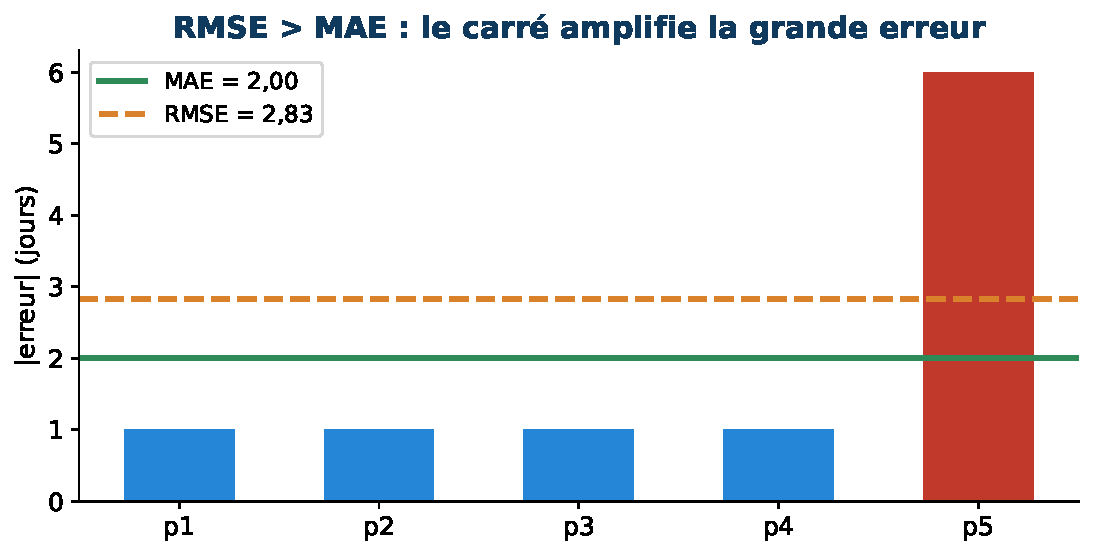
\includegraphics[width=0.62\linewidth]{f5_mae_rmse}
\vspace{-2pt}

{\small Cinq patients, erreurs absolues $(1,1,1,1,6)$. MAE $= 10/5 = \mathbf{2{,}00}$ jours. RMSE $= \sqrt{(1+1+1+1+36)/5} = \sqrt{8} = \mathbf{2{,}83}$ jours. La cinquième erreur pèse $36$ dans les carrés contre $6$ dans les valeurs absolues : un seul patient raté tire la RMSE bien au-dessus de la MAE.}
\end{frame}

\begin{frame}{Mesurer avec la MAE, optimiser avec la MSE}
\begin{columns}[c]
\column{0.45\linewidth}
\centering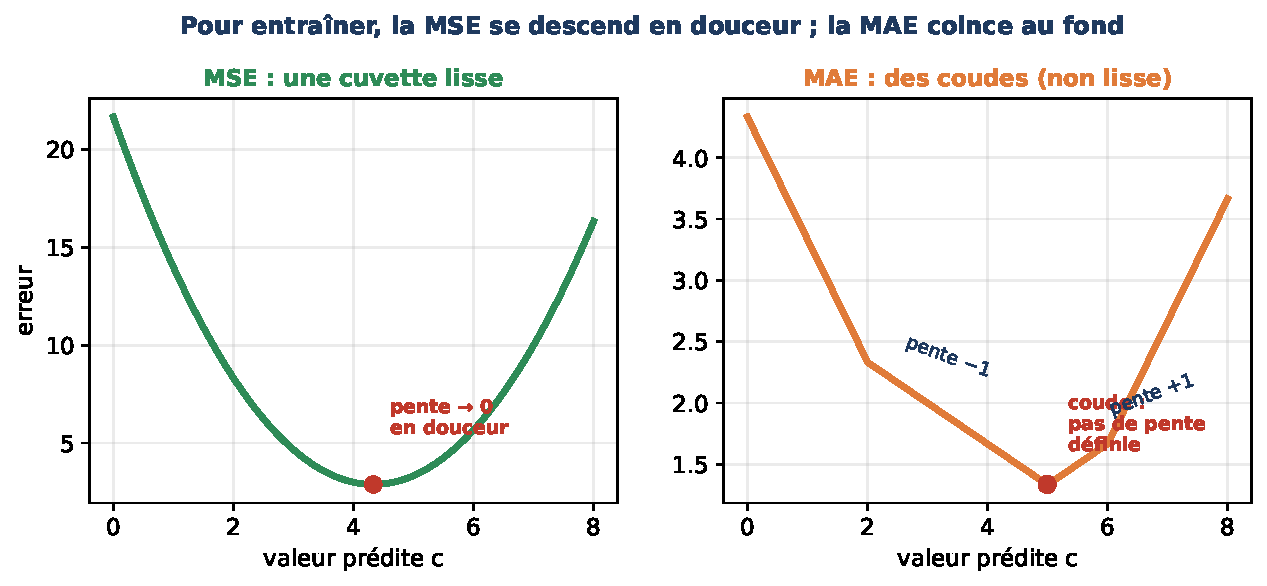
\includegraphics[width=\linewidth]{f5_mae_vs_mse_opt}
\column{0.55\linewidth}
\begin{ucadret}[Deux rôles, deux choix]
\begin{itemize}\small
  \item \textbf{MAE} : toutes les erreurs au même tarif, robuste aux valeurs extrêmes et lisible en jours — mais sa courbe forme un \textbf{coude} au minimum (pente indéfinie), malcommode à minimiser.
  \item \textbf{MSE} : surtaxe les grosses erreurs (sensible aux extrêmes) — mais sa cuvette est \textbf{lisse et dérivable partout}, facile à descendre.
  \item En pratique : \textbf{entraîner} en minimisant la MSE, puis \textbf{rapporter} MAE et RMSE (lecture en jours).
\end{itemize}
\end{ucadret}
\end{columns}
\vspace{1pt}

{\scriptsize La MSE (gauche) a une pente qui s'annule en douceur ; la MAE (droite) a un coude où la pente saute de $-1$ à $+1$ sans passer par $0$.}
\end{frame}

\begin{frame}{Le R², formellement}
\begin{ucaddef}[L'idée en une phrase]
{\small Le \textbf{R²} compare le modèle au prédicteur le plus paresseux — toujours répondre la moyenne $\bar y$ — et mesure quelle part de l'erreur de ce paresseux le modèle fait disparaître.}
\end{ucaddef}
\ucadformula{R^2 \;=\; 1 \;-\; \frac{\sum_i (y_i - \hat y_i)^2}{\sum_i (y_i - \bar y)^2}}
{\small Numérateur : l'erreur (quadratique) du modèle ; dénominateur : celle de la moyenne. $R^2 = 1$ : prédiction parfaite ; $R^2 = 0$ : pas mieux que la moyenne ; $R^2 < 0$ : \emph{pire} que la moyenne — toujours possible sur le test, et toujours mauvais signe. Sans unité, le R² complète la MAE/RMSE qui, elles, parlent en jours.}
\end{frame}

\begin{frame}{Exemple — le R² du jouet, décomposé}
\begin{ucadex}[Les deux sommes sont déjà connues]
{\small Pour la droite $\hat y = 0{,}5 + 1{,}1x$ : la somme des carrés des résidus vaut $0{,}70$ (calcul de la MSE). Pour la moyenne : $6{,}75$ (l'exercice de la droite plate).
\[ R^2 = 1 - \frac{0{,}70}{6{,}75} = 1 - 0{,}104 = \mathbf{0{,}896} \]
La droite efface $89{,}6\,\%$ de l'erreur quadratique du prédicteur-moyenne. \texttt{r2\_score} de \texttt{scikit-learn} retourne la même valeur — et c'est ce que \texttt{score()} calcule pour tout régresseur.}
\end{ucadex}
\end{frame}

\begin{frame}{Exercice — interpréter trois R²}
\begin{ucadrec}[Énoncé]
{\small Trois modèles de la durée d'hospitalisation affichent, sur le \emph{test} : $R^2_A = 0{,}90$, $R^2_B = 0{,}00$, $R^2_C = -0{,}30$. Interpréter chaque valeur en une phrase.}
\end{ucadrec}
\pause
\begin{ucadex}[Correction]
{\small $A$ supprime $90\,\%$ de l'erreur quadratique de la moyenne : excellent sur ces données. $B$ ne fait \emph{pas mieux} que répondre $\bar y$ partout : il n'a rien appris d'utile. $C$ fait \emph{pire} que la moyenne — typique d'un modèle sur-ajusté à son train, ou d'une fuite dans le protocole. Réflexe : un R² s'annonce toujours \emph{avec} la MAE ou la RMSE, qui parlent en jours.}
\end{ucadex}
\end{frame}

\begin{frame}[fragile]{La régression de la durée d'hospitalisation}
\begin{lstlisting}
from sklearn.linear_model import LinearRegression
from sklearn.metrics import mean_absolute_error, r2_score

X = df[["age", "glycemie", "hemoglobine", "fievre", "saison"]]
y = df["duree_hospit_j"]              # cible continue, en jours
X_tr, X_te, y_tr, y_te = train_test_split(X, y, test_size=0.2,
                                          random_state=42)
modele = LinearRegression().fit(X_tr, y_tr)
y_pred = modele.predict(X_te)
\end{lstlisting}
{\small Le protocole de la Séance 3, à deux différences près : la cible est \texttt{duree\_hospit\_j} (pas de \texttt{stratify} — il ne concerne que les classes), et les métriques changent de famille.}
\end{frame}

\begin{frame}{Le bilan chiffré de la séance}
\begin{ucadex}[Trois modèles sur le test]
{\small \begin{center}\renewcommand{\arraystretch}{1.1}\begin{tabular}{l|ccc}
modèle & MAE (jours) & RMSE (jours) & R²\\\hline
baseline (moyenne) & $2{,}17$ & — & $-0{,}001$\\
arbre de régression, prof. 5 & $1{,}45$ & — & $0{,}533$\\
\textbf{régression linéaire} & $\mathbf{1{,}35}$ & $\mathbf{1{,}67}$ & $\mathbf{0{,}598}$\\
\end{tabular}\end{center}
Le linéaire se trompe de $1{,}35$ jour en moyenne et efface $60\,\%$ de l'erreur de la baseline. Il \textbf{devance l'arbre} de la Séance 3 : la durée est fabriquée par des effets additifs (glycémie, saison...), terrain naturel d'un modèle linéaire — chaque famille de modèles a ses terrains.}
\end{ucadex}
\end{frame}

\begin{frame}{Le diagnostic visuel : prédit contre réel, résidus}
\begin{columns}[c]
\column{0.37\linewidth}
\centering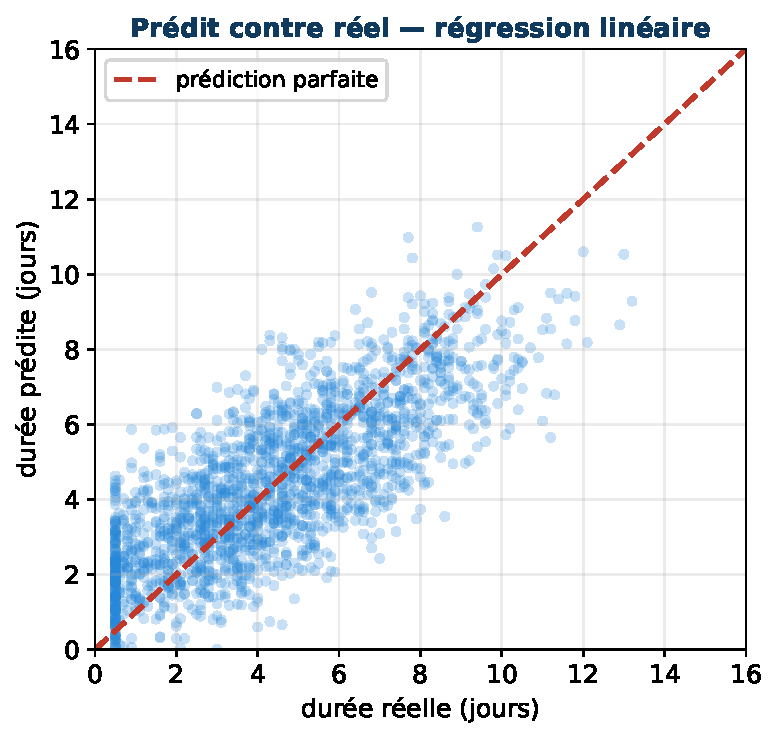
\includegraphics[width=\linewidth]{f5_pred_vs_true}
\column{0.60\linewidth}
\centering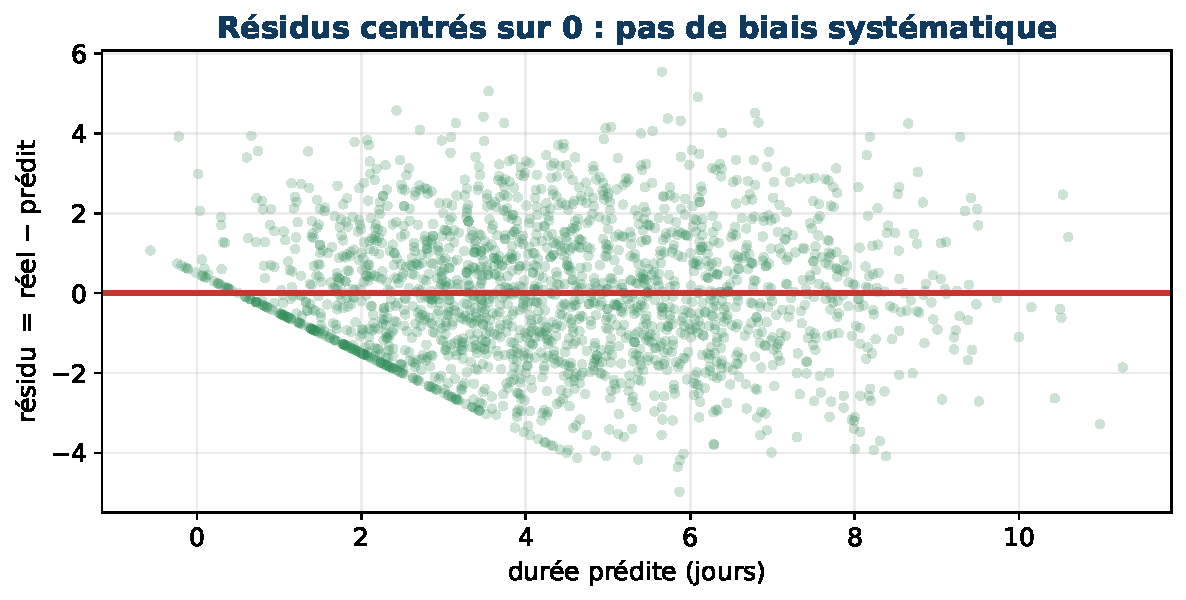
\includegraphics[width=0.94\linewidth]{f5_residuals}
\end{columns}
\vspace{1pt}

{\scriptsize À gauche : le nuage longe la diagonale « prédiction parfaite » — avec un écrasement sur les longues durées, que le modèle sous-estime. À droite : les résidus en fonction du prédit, centrés sur $0$ (pas de biais systématique). Toute \emph{forme} dans ce nuage — courbure, entonnoir — signalerait un motif que la droite n'a pas capté.}
\end{frame}

% #####################################################################
\section[Le degré]{Le degré : sous- et sur-ajustement}

\begin{frame}{Au-delà de la droite : l'expansion polynomiale}
\begin{ucaddef}[Définition]
{\small Quand la relation est \emph{courbe}, on garde le modèle linéaire mais on enrichit les \textbf{entrées} : aux côtés de $x$, on ajoute $x^2, x^3, \dots, x^p$ comme nouvelles colonnes. La droite, tracée dans cet espace enrichi, devient une courbe dans l'espace d'origine.}
\end{ucaddef}
\ucadformula{\varphi_p(x) = \big(x,\, x^2,\, \dots,\, x^p\big) \qquad\quad \hat y = b + w_1 x + w_2 x^2 + \cdots + w_p x^p}
{\small Exemple : $\varphi_3(2) = (2, 4, 8)$. Le modèle reste \emph{linéaire en ses poids} — équation normale et descente de gradient s'appliquent inchangées. Le \textbf{degré} $p$ devient un bouton de complexité, exactement comme la profondeur de l'arbre en Séance 3 — et \texttt{PolynomialFeatures} est une étape de Pipeline, comme tout prétraitement de la Séance 4.}
\end{frame}

\begin{frame}{L'analogie : une règle qu'on laisse se courber}
\begin{ucadfront}[Comprendre la régression polynomiale]
{\small Une droite, c'est une règle \textbf{rigide} : elle ne peut pas épouser une courbe. Lui ajouter $x^2, x^3, \dots$ revient à remplacer la règle par une \textbf{tige souple} : plus on autorise de courbures (le degré $p$), plus elle suit les points. Trop souple, elle ondule pour passer par \emph{chaque} point, jusqu'à suivre le bruit — c'est le sur-ajustement.}
\end{ucadfront}
\figslideb{0.52}{f5_poly_bend}{La droite rigide (rouge) rate la courbure des points ; le polynôme de degré $3$ (vert), plus souple, la suit.}
\end{frame}

\begin{frame}{Trois degrés, trois destins}
\centering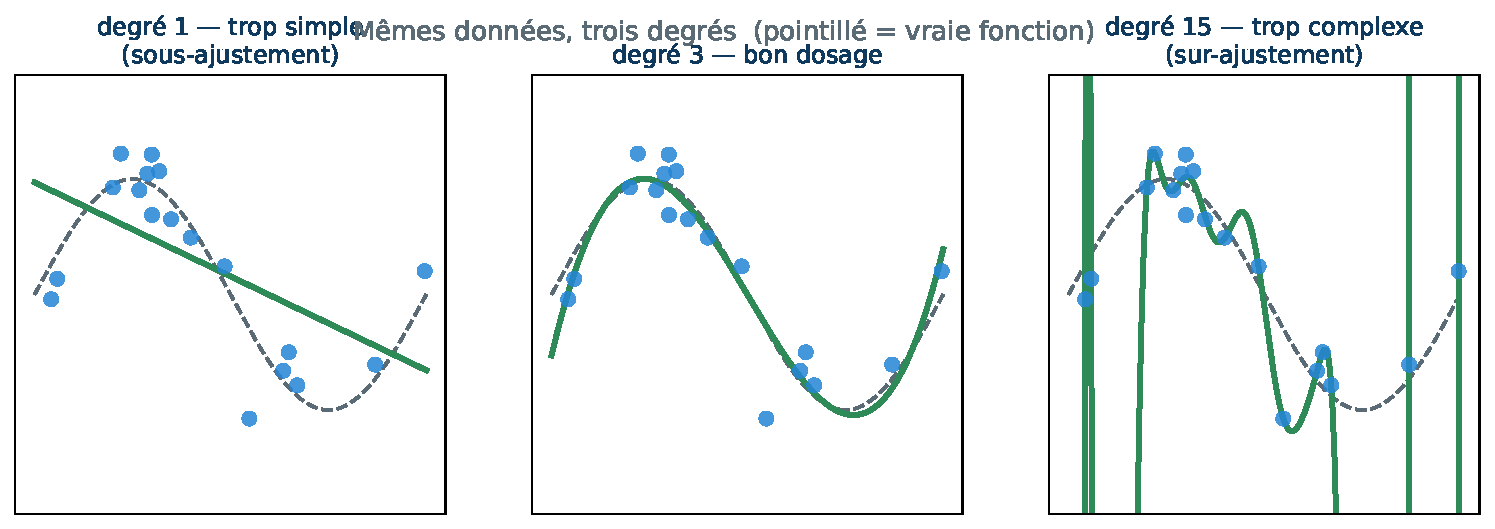
\includegraphics[width=0.94\linewidth]{f5_threefits}
\vspace{-1pt}

{\small Trente points tirés d'une sinusoïde bruitée (pointillés : la vraie fonction). Le degré 1 est trop rigide pour la courbure : \textbf{sous-ajustement}. Le degré 3 épouse la forme. Le degré 15 passe presque par chaque point — il apprend le \emph{bruit} : \textbf{sur-ajustement}. Le vocabulaire de la Séance 3 s'applique tel quel ; seul le bouton a changé.}
\end{frame}

\begin{frame}{L'erreur d'entraînement est une flatteuse}
\begin{columns}[c]
\column{0.50\linewidth}
\begin{ucadex}[Le piège chiffré]
{\small Sinusoïde (18 train, 12 validation) :
\begin{center}\footnotesize\renewcommand{\arraystretch}{1.1}\begin{tabular}{l|cc}
 & RMSE train & RMSE val.\\\hline
degré 3 & $0{,}244$ & $\mathbf{0{,}287}$\\
degré 15 & $\mathbf{0{,}094}$ & $1386$\\
\end{tabular}\end{center}
Au train seul, le degré 15 semble « deux fois et demie meilleur » ; en validation il est \textbf{cinq mille fois pire}. Seule une donnée \emph{jamais vue} dit la vérité.}
\end{ucadex}
\column{0.50\linewidth}
\centering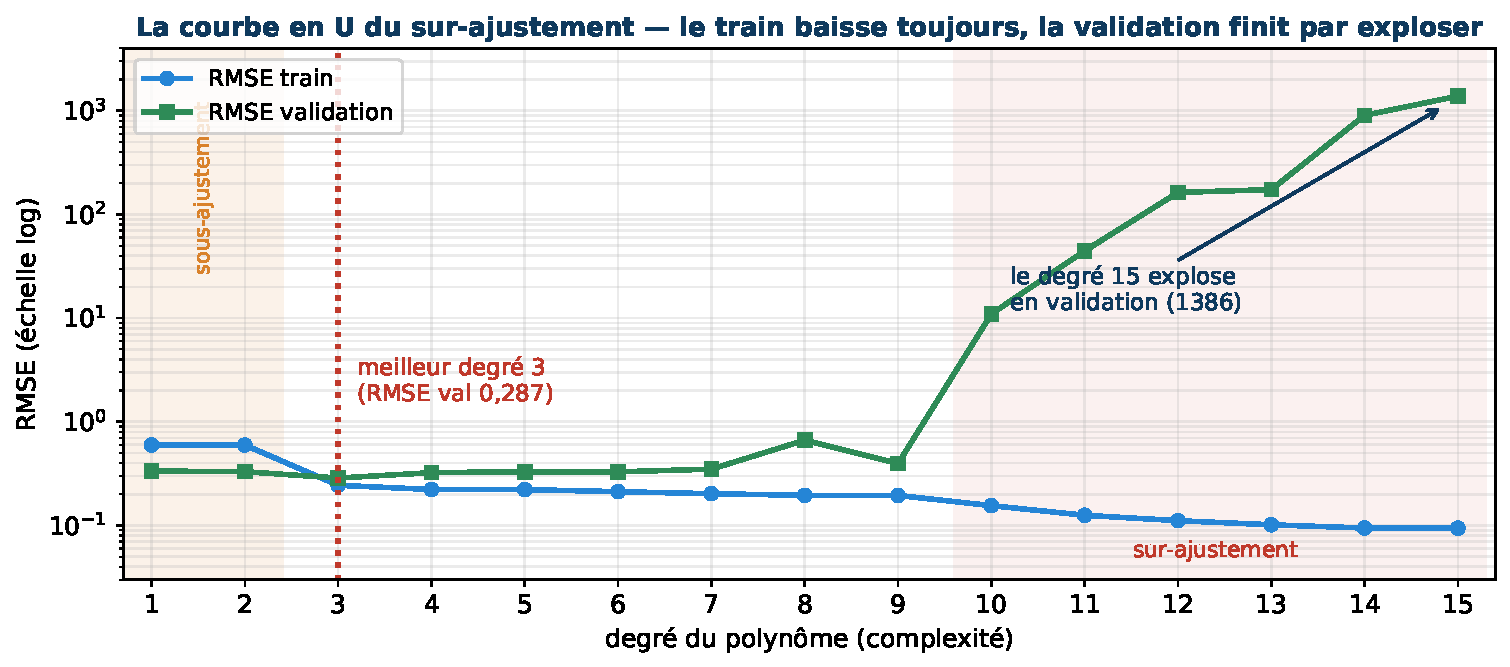
\includegraphics[width=\linewidth]{f5_ucurve}
\end{columns}
\vspace{1pt}

{\scriptsize Degrés 1 à 15 : la RMSE train (bleu) descend \emph{toujours} ; la validation (vert) creuse au degré 3, puis explose. Choisir la complexité, c'est chercher le creux du U — jamais le bas de la courbe bleue.}
\end{frame}

\begin{frame}{Exercice — diagnostiquer par la paire de scores}
\begin{ucadrec}[Énoncé]
{\small Trois polynômes sur un même jeu : $A$ — RMSE train $0{,}60$, validation $0{,}62$ ; $B$ — train $0{,}24$, validation $0{,}29$ ; $C$ — train $0{,}09$, validation $14{,}5$. Diagnostiquer chacun (sous-ajusté, bien dosé, sur-ajusté) et choisir le modèle à déployer.}
\end{ucadrec}
\pause
\begin{ucadex}[Correction]
{\small $A$ : deux erreurs \emph{hautes et proches} — trop simple, sous-ajustement. $C$ : train minuscule, validation catastrophique — mémorisation, sur-ajustement. $B$ : erreurs basses et voisines — le bon dosage, c'est lui que l'on déploie. Le diagnostic se lit toujours dans l'\emph{écart} entre les deux scores, jamais dans le train seul.}
\end{ucadex}
\end{frame}

% #####################################################################

\section[Ridge]{Ridge : dompter le sur-ajustement}

\begin{frame}{L'idée : punir les coefficients géants}
\begin{ucadex}[L'empreinte du sur-ajustement]
{\small Le polynôme de degré 15 qui explose en validation cache un symptôme spectaculaire : son plus grand coefficient atteint $\mathbf{9{,}2}$ \textbf{milliards}. Pour zigzaguer entre 18 points, la courbe a besoin de pentes vertigineuses qui se compensent au micron près — c'est cela, mémoriser du bruit.}
\end{ucadex}
\begin{ucaddef}[L'idée en une phrase]
{\small \textbf{Ridge} ajoute à l'erreur une \textbf{pénalité qui grandit avec la taille des coefficients} — comme un \emph{élastique} reliant chaque coefficient à zéro : le poids ne glisse plus tout à fait jusqu'au minimum MSE, il s'en \emph{approche} en restant plus près de $0$. Le modèle ne garde alors un gros coefficient que s'il réduit \emph{vraiment} l'erreur ; les superflus sont tirés vers zéro, et la course aux pentes géantes n'est plus rentable.}
\end{ucaddef}
\end{frame}

\begin{frame}{Ridge, formellement}
\begin{ucaddef}[Définition]
{\small \textbf{Ridge} minimise la MSE \emph{augmentée} d'une pénalité proportionnelle à la somme des carrés des poids, dosée par $\alpha \geq 0$.}
\end{ucaddef}
\ucadformula{J_{\text{ridge}}(b,\mathbf{w}) \;=\; \underbrace{\frac{1}{n}\sum_{i=1}^{n}\big(y_i - \hat y_i\big)^2}_{\text{coller aux données}} \;+\; \alpha \underbrace{\sum_{j=1}^{d} w_j^2}_{\text{rester sobre}}}
{\small Les deux termes tirent en sens contraires et $\alpha$ arbitre : $\alpha = 0$ redonne les moindres carrés ordinaires ; $\alpha$ immense écrase tous les poids vers $0$ (la droite plate). $b$ n'est pas pénalisé — le niveau de base n'est pas un luxe. La cuvette reste une cuvette : équation normale et descente de gradient s'adaptent sans douleur.}
\end{frame}

\begin{frame}{Comment la pénalité agit}
\begin{ucadfront}[Comment ça pénalise, concrètement]
{\small On ne minimise plus l'erreur seule, mais la somme \emph{erreur} $+\,\alpha\sum_j w_j^2$. Augmenter un poids $w_j$ a donc deux effets opposés : cela peut \textbf{baisser l'erreur} (gain), mais cela \textbf{fait toujours monter la pénalité} (coût, en $w_j^2$). À l'optimum, chaque poids s'arrête là où le gain marginal sur l'erreur \emph{égale} le coût marginal de la pénalité. Un poids inutile n'apporte aucun gain : seul son coût compte, et il est poussé vers $0$.}
\end{ucadfront}
{\small Le carré rend la pénalité \emph{progressive} : doubler un coefficient quadruple son coût. Les très gros poids — ceux du sur-ajustement — deviennent les plus chers, donc les premiers sabrés. C'est $\alpha$ qui fixe le prix : plus il est grand, plus les coefficients sont comprimés.}
\end{frame}

\begin{frame}{Le degré 15 dompté : avant et après}
\begin{columns}[c]
\column{0.54\linewidth}
\begin{ucadex}[Le même polynôme sous quatre régimes]
{\small Degré 15 sur la sinusoïde, coefficients standardisés :
\begin{center}\footnotesize\renewcommand{\arraystretch}{1.0}\begin{tabular}{c|cc}
$\alpha$ & plus grand $|w_j|$ & RMSE val.\\\hline
$0$ & $9{,}2$ milliards & $1386$\\
$0{,}001$ & $7{,}8$ & $0{,}31$\\
$\mathbf{0{,}1}$ & $1{,}8$ & $\mathbf{0{,}27}$\\
$100$ & $0{,}05$ & $0{,}51$\\
\end{tabular}\end{center}
À $\alpha = 0{,}1$, le degré 15 régularisé ($0{,}27$) bat même le meilleur degré non pénalisé ($0{,}287$).}
\end{ucadex}
\column{0.46\linewidth}
\centering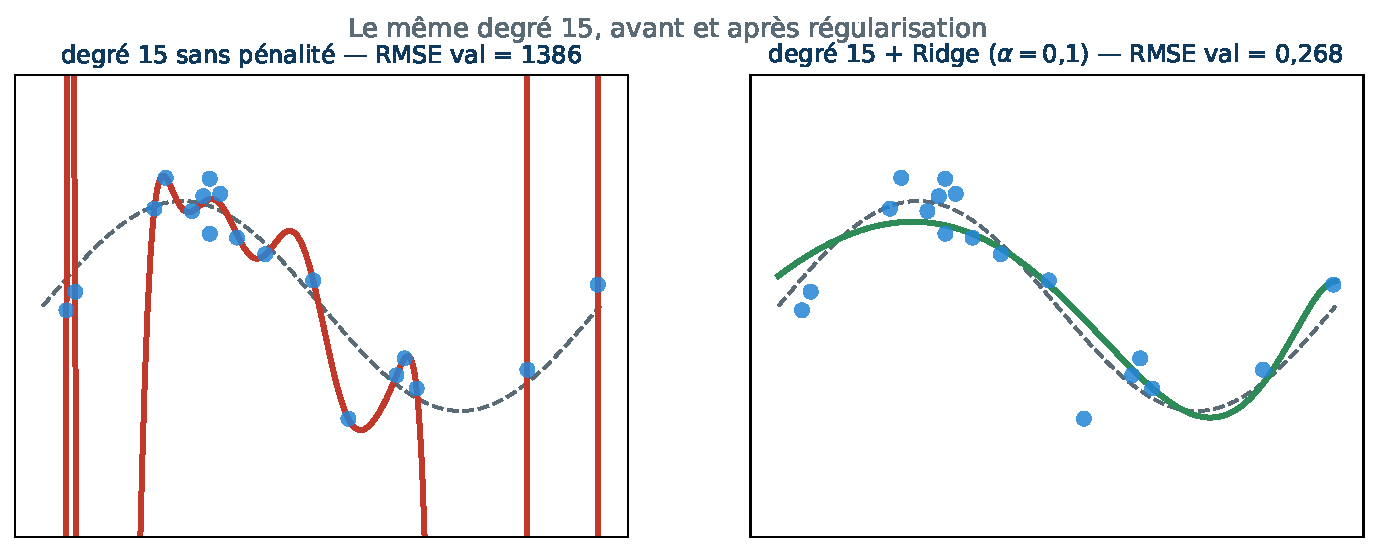
\includegraphics[width=\linewidth,height=0.50\textheight,keepaspectratio]{f5_ridge}
\end{columns}

{\scriptsize Même degré 15 : sans pénalité la courbe s'emballe ; avec $\alpha = 0{,}1$ elle retrouve la sinusoïde.}
\end{frame}

\begin{frame}{Exercice — le rôle de $\alpha$}
\begin{ucadrec}[Énoncé]
{\small \textbf{(a)} Vers quel modèle tend Ridge quand $\alpha \to \infty$ ? \textbf{(b)} Un collègue règle $\alpha$ en choisissant la valeur qui minimise la RMSE \emph{d'entraînement}. Quelle valeur va-t-il systématiquement choisir, et pourquoi est-ce une erreur ?}
\end{ucadrec}
\pause
\begin{ucadex}[Correction]
{\small \textbf{(a)} Tous les $w_j$ sont écrasés vers $0$ : il reste $\hat y = b$, la droite plate à hauteur de la moyenne — le sous-ajustement maximal. \textbf{(b)} $\alpha = 0$ : toute pénalité ne peut qu'augmenter l'erreur de train, puisqu'elle contraint l'ajustement. Le bon $\alpha$ se choisit sur la \textbf{validation} — le train, flatteur, vote toujours pour la complexité maximale.}
\end{ucadex}
\end{frame}

\begin{frame}{Piège — régulariser sans standardiser}
\begin{ucadpiege}[Une pénalité injuste]
{\small La pénalité $\alpha\sum w_j^2$ compare les poids entre eux — elle n'a de sens que si les variables parlent la \textbf{même monnaie}. Sans standardisation, une variable d'échelle minuscule a besoin d'un grand poids pour peser : Ridge la punit injustement. Le Pipeline de la Séance 4 s'impose : \texttt{StandardScaler} \emph{puis} \texttt{Ridge}, le scaler ajusté sur le train seulement.}
\end{ucadpiege}
{\small Troisième rendez-vous de la standardisation : le kNN (distances), la descente de gradient (cuvette ronde), Ridge (pénalité équitable). Ce n'est pas un détail de cuisine — c'est une pièce du contrat de validité des modèles.}
\end{frame}

\begin{frame}{Une variante : Lasso (et Elastic Net)}
\begin{ucaddef}[L'idée en une phrase]
{\small \textbf{Lasso} suit la même idée que Ridge — pénaliser la taille des coefficients — mais sur la \emph{somme des valeurs absolues} au lieu des carrés. Conséquence frappante : là où Ridge \emph{rétrécit} sans jamais annuler, Lasso pousse certains coefficients \textbf{exactement à zéro} et fait donc de la \textbf{sélection de variables}.}
\end{ucaddef}
\ucadformula{J_{\text{lasso}} = \frac{1}{n}\sum_{i}\big(y_i-\hat y_i\big)^2 \;+\; \alpha\sum_{j=1}^{d}\,\lvert w_j\rvert \qquad\text{(Ridge : } \alpha\sum_j w_j^2\text{)}}
{\small Image : Ridge \emph{baisse les salaires de tous}, Lasso \emph{licencie les moins utiles}. On prend Ridge quand toutes les variables comptent un peu (stabiliser le modèle), Lasso quand on en soupçonne beaucoup d'inutiles (modèle simple, interprétable). Un compromis, l'\emph{Elastic Net}, combine les deux pénalités. Les trois s'emploient comme \texttt{LinearRegression}, dans un Pipeline après le \texttt{StandardScaler}, et se règlent par $\alpha$ en validation (le creux du U).}
\end{frame}

\section{Synthèse}

\begin{frame}{Le protocole de régression}
\begin{ucadret}[De bout en bout]
{\small \textbf{1.} Cible continue identifiée ($y \in \mathbb{R}$, en jours) $\to$ \textbf{2.} split train/test $\to$ \textbf{3.} Pipeline (imputation, standardisation si descente ou Ridge) $\to$ \textbf{4.} \texttt{LinearRegression} — ou \texttt{Ridge}, ou \texttt{SGDRegressor} selon l'échelle du problème $\to$ \textbf{5.} MAE + RMSE + R² \emph{sur le test}, comparés à la baseline-moyenne $\to$ \textbf{6.} graphe des résidus $\to$ \textbf{7.} si complexité à régler (degré, $\alpha$) : choisir au creux du U de \emph{validation}, jamais au train.}
\end{ucadret}
\end{frame}

\begin{frame}{À retenir — Séance 5}
\begin{ucadret}[L'essentiel]
\begin{itemize}\small
  \item La régression prédit un \textbf{réel} ; le modèle linéaire le fait par somme pondérée : $\hat y = b + \mathbf{w}\cdot\mathbf{x}$, et ses coefficients se lisent en clair.
  \item La \textbf{MSE} définit la meilleure droite ; sa cuvette admet un minimum \textbf{exact} : l'équation normale $\hat\theta = (\tilde X^{\top}\tilde X)^{-1}\tilde X^{\top}y$.
  \item La \textbf{descente de gradient} atteint le même minimum par pas successifs $\theta \leftarrow \theta - \eta\nabla J$ ; le pas $\eta$ arbitre entre lenteur et divergence. C'est l'algorithme d'apprentissage universel du ML.
  \item \textbf{MAE} et \textbf{RMSE} parlent en jours (la RMSE surtaxe les grandes erreurs) ; le \textbf{R²} compare à la baseline-moyenne.
  \item Le degré polynomial est un bouton de complexité : le train flatte, la \textbf{validation} tranche (courbe en U).
  \item \textbf{Ridge} ($+\,\alpha\sum w_j^2$) rétrécit tous les coefficients ; \textbf{Lasso} ($+\,\alpha\sum|w_j|$) en annule certains et sélectionne les variables. Standardiser d'abord, régler $\alpha$ en validation.
\end{itemize}
\end{ucadret}
\end{frame}

\begin{frame}{Pièges fréquents}
\begin{itemize}\small
  \item Lire les coefficients de variables d'échelles différentes comme des importances comparables.
  \item Confondre association et causalité dans un poids $w_j$.
  \item Annoncer un R² sans MAE/RMSE — ou l'inverse : les deux familles se complètent.
  \item Choisir degré ou $\alpha$ sur l'erreur d'\emph{entraînement} : elle vote toujours pour la complexité maximale.
  \item Lancer une descente de gradient (ou Ridge) sur des variables non standardisées.
  \item Oublier que le prétraitement s'ajuste sur le train seul — la fuite de la Séance 4 guette aussi la régression.
  \item Un R² négatif sur le test n'est pas un bug de \texttt{scikit-learn} : le modèle fait pire que la moyenne.
\end{itemize}
\end{frame}

\begin{frame}{Prochaine séance}
\begin{ucadfront}[Séance 6 — Classifier et choisir ses métriques]
{\small Retour aux classes, mais en profondeur. Le modèle linéaire d'aujourd'hui en est le \textbf{cœur} : la \emph{même} somme pondérée $z = b + \mathbf{w}\cdot\mathbf{x}$, cette fois passée dans une \textbf{sigmoïde} pour devenir une probabilité — c'est la régression \emph{logistique}. Puis la matrice de confusion, precision, recall, F1, les courbes ROC, et le cas qui fâche : prédire le paludisme, présent chez $11{,}8\,\%$ des patients seulement, là où l'accuracy devient une métrique menteuse.}
\end{ucadfront}
\end{frame}

\begin{frame}{Références}
\begin{itemize}\small
  \item James, Witten, Hastie, Tibshirani — \emph{An Introduction to Statistical Learning}, 2\textsuperscript{e} éd., Springer, 2021.
  \item Géron — \emph{Hands-On Machine Learning}, 3\textsuperscript{e} éd., O'Reilly, 2022.
  \item Müller, Guido — \emph{Introduction to Machine Learning with Python}, O'Reilly, 2016.
  \item Cours : University of Washington CSE 446 ; Stanford CS229.
\end{itemize}
\end{frame}

\end{document}
